%%%%%%%%%%%%%%%%%%%%%%%%%%%%%%%%%%%%%%%%%%%%%%%%%%%%%%%%%%%%%%%%%%%%%%%%%%%%%
%%% A Dependency Network+Weigthed Kernel Approach for Feature Selection
%%% Proposal for a MSc Project
%%% Nestor Rodriguez + Sergio A. Rojas (c) 2010
%%%
%%% Chapter 2: Formulation
%%%%%%%%%%%%%%%%%%%%%%%%%%%%%%%%%%%%%%%%%%%%%%%%%%%%%%%%%%%%%%%%%%%%%%%%%%%%%
\section{Problem, Motivation and Research Hypothesis}
\subsection{Problem and Motivation}
\label{sec:formulation}

Feature subset selection (FSS) is a machine learning technique for dimensionality reduction in datasets where irrelevant or noisy variables may appear. It is useful in problems where few from a big set of observed variables explain a given pattern in classification, prediction or clustering of data cases (e.g. diagnosis of a disease, market analysis, image segmentation, etc.), and therefore it allows for an expert to focus on data that is really important, reducing the expenditure of costly or time-consuming experiments.  

To illustrate the problem, consider the situation where an insurance company is evaluating the factors that have an impact on people's overweight conditions that lead to claims in illness insurance policies. Upon registration, they collect information of both parents' weight and birthday. They want to know which of these variables are related to the development of the condition. Now let us suppose that one-year time is required by an insurance analyst to process the information of just one variable. Then it would be desirable to discard irrelevant variables in order to save him valuable time. An FSS method could help to select the relevant ones.

\begin{figure}[h]
	\centering
		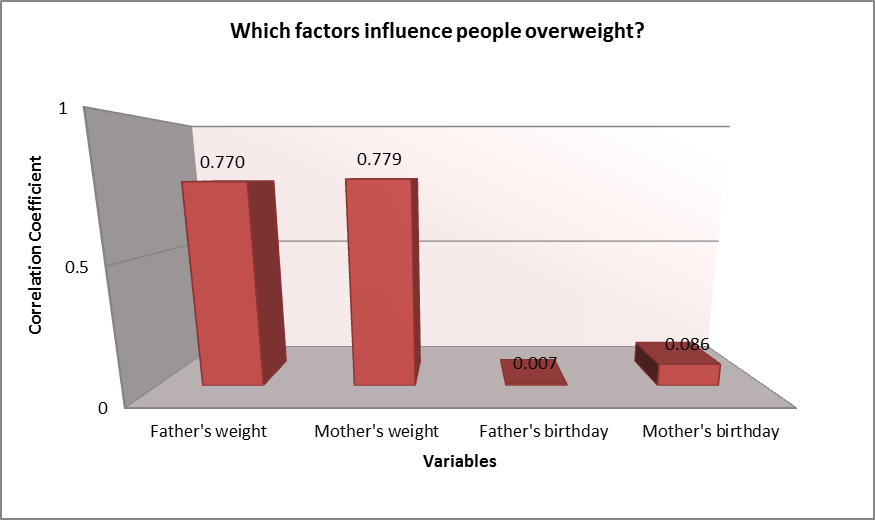
\includegraphics{Images/example01}
	\caption[Correlation analysis of input variables in relation to overweight conditions of insurance customers.]%
	{Correlation analysis of input variables in relation to overweight conditions of insurance customers (for the fictional example in the text).}
	\label{fig:im01}
\end{figure}

Figure \ref{fig:im01} depicts the result of applying a correlation-based feature selection method on this fictional problem; it is evident that half of the variables, namely those related to birth dates, are irrelevant and can be ignored for the problem of interest. Thus, dimensionality reduction may provide insights in data mining tasks, yielding a better understanding of objects or phenomena behavior and is useful to speed up data analysis and to improve generalization performance. For instance, in the previous insurance company example, Figure \ref{fig:im08} shows how sample cases can be now rendered in the 2D space obtained with the relevant variables; they can be easily discriminated with a simple hyperplane. By focusing on those two relevant variables, the analyst would have saved two precious years of working time and the company two equally valuable years of salary payments. 

\begin{figure}[h]
	\centering
		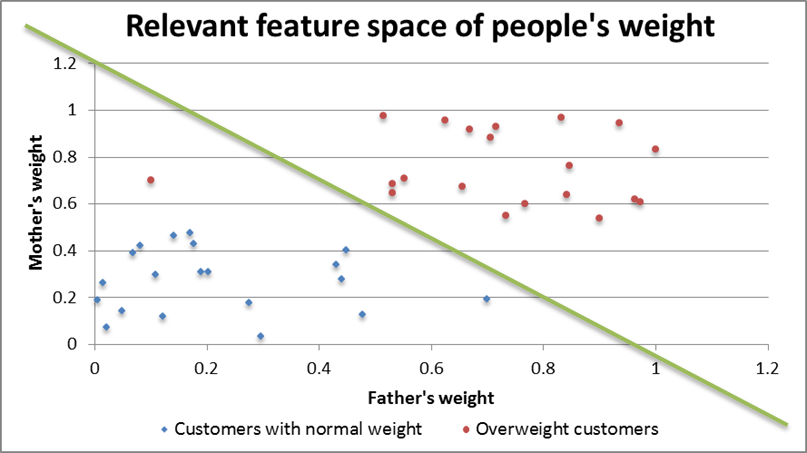
\includegraphics{Images/example02.png}
	\caption{Using relevant features customers can be easily segmented with a simple linear function.}
	\label{fig:im08}
\end{figure}

Some FSS techniques assume variables are independent.  This assumption might not be appropriate for some real world problem since variables may influence others and these interactions are usually hidden.  A good example is in the field of bioinformatics where experts analyze proteins relevance in diseases to design inhibitory vaccines; using state-of-the-art high-throughput technologies (e.g. mass-spectometry\cite{lipton08}) they are able to collect large amounts of data about activation of protein mechanisms, but the information about how these interactions occur is unknown or difficult to obtain, not to mention that just a few proteins from a large proteomic spectrum would be related to the activation of the disease. 

The independent assumptions (univariate FSS methods, see section \ref{sec:feat1}) are very popular because of their low computational cost\cite{larranaga08} but they do not provide additional insights about data relationships.  On the other hand, missing information about those dependencies may affect negatively the prediction accuracy of the feature subset.  As an alternative approach, multivariate FSS methods search for feature subsets and possible dependency relationships between them at the cost of an increase in computational complexity (recall that FSS is a combinatorial problem known to be NP-Hard \cite{guyon03,rojas05}). The challenge is then to design novel feature selection methods that take advantage of multivariate power combined with high-accuracy classifiers to obtain improved prediction and explanatory performance.

On the other hand, kernel classifiers have recently emerged as powerful high-accuracy classifiers with robust generalization abilities \cite{cristianini04}.  They use linear functions to perform classification, allowing for non-linear discriminatory borderlines in the input space by means of a kernel function. This function is a mapping of similarity measures in a transformed space where nonlinearities can be solved linearly. Two widely used kernel functions are the RBF kernel and the polynomial kernel (Eq.(\ref{eq:eq01}) and Eq.(\ref{eq:eq02}) respectively):

\pdfcomment[avatar={reviewer}, id=5]{5.1 Whenever a mathematical symbol is used, it should be clearly defined. }
\pdfreply[avatar=me, id=50, replyto=5]{Symbols in equations and algorithms were clearly defined.}
\begin{equation}
	K_{\sigma}(\bar{x},\bar{z}) = \text{exp}\Big( -\sigma\sum_{k} (x_k-z_k)^2 \Big)
	\label{eq:eq01}
\end{equation} and
\begin{equation}
	K_d(\bar{x},\bar{z}) = \langle \bar{x}, \bar{z} \rangle^d,
	\label{eq:eq02}
\end{equation} where \(\bar{x}, \bar{z} \in X\), \(X \subseteq \mathbb{R}^D \) represents the input space and {\scriptsize $D$ } the number of variables or dimensions.  The parameter \(\sigma\) and \(d\) define the width of the RBF and polynomial kernel respectively.  Modified weighted versions of these kernels introduce scale factors \(\bar{w} = \{w_1...w_\ell\}\) to weight the amount that each dimension contributes to the total computation\cite{vapnik02}.  The weighted RBF and weighted polynomial kernels are then defined as Eq.(\ref{eq:eq03}) and (\ref{eq:eq04}):

\begin{equation}
	K_{\sigma}(\bar{x},\bar{z}) = \text{exp}\Big( -\sigma \sum_{k}^{\ell} w_k(x_k-z_k)^2 \Big)
	\label{eq:eq03}
\end{equation} and

\begin{equation}
	K_{d}(\bar{x},\bar{z}) = \Big( \sum_{k}^{\ell} w_k(x_k \cdot z_k) \Big)^d.
	\label{eq:eq04}
\end{equation}

Some FSS methods have been proposed in connection with kernel functions, for instance the weighted kernels in Eq. (\ref{eq:eq03}) and (\ref{eq:eq04}) have been used to define a FSS embedded method (the weigthed kernel iterative estimation of relevance algorithm, wKIERA\cite{rojas08}).  The idea in this case is to consider the weight vector \(\bar{w}\) of the kernel as a relevancy estimator of input variables. The vector is tuned by a univariate estimation of distribution algorithm \cite{larranaga01} which iteratively refines the distribution by a population-based technique inspired in genetic algorithms (GA)\cite{goldberg89}. The accuracy of the kernel classifier coupled with the weight vector candidates is taken as the fitness measure of the GA.  The authors showed promising results of this algorithm in selecting relevant variables in a number of different classification tasks, including problems with linear and non-linear hypothesis targets. This FSS method however, is designed on the basis of the independent assumption mentioned above and consequently does not provide the power of explanation of multivariate methods and does not account for information of relationship between the variables. One of the motivations of this thesis proposal is to build upon this method and design a refined version that incorporates techniques for multivariate feature selection within an embedded population-based stochastic algorithm. Dependency networks, also known as belief or Bayes networks \cite{heckerman99}, would be preliminary chosen to represent how variables depend and influence each other, and one of the goals of the thesis is to design and new algorithms to perform relevance estimation within such framework and to make feasible the approach. 

Finally, it is worth to note that the work by \cite{larranaga00FSS} propose a FSS multivariate method that accounts for dependencies between variables by estimating belief networks. Their approach however is a wrapper method (see section \ref{sec:feat1}) and they do not incorporate the powerfulness of nonlinear kernel classifiers. We will however review this study, and as far as possible compare the different approaches.

\subsection{Research Hypothesis} 
\pdfcomment[avatar={reviewer}, id=1]{It is convenient to establish the problem as a research hypothesis to be tested, in order to clarify
 the contributions and facilitate the evaluation of the research project.}
 \pdfreply[id=10,avatar={me},replyto=1]{This section presents the missing research hypothesis.}

We will consider the following research hypothesis: Given a set of observations taken from a particular phenomenon where dependencies among variables exist but are hidden, it is feasible to select a subset of variables that are relevant in a classification task with a method that combines iterative estimation of dependency networks coupled with weighted-kernel classifiers, in order to produce a predictor model that improves the understanding of the problem domain when compared with other techniques based on independence assumptions.